\begin{figure}[htbp]
\centering
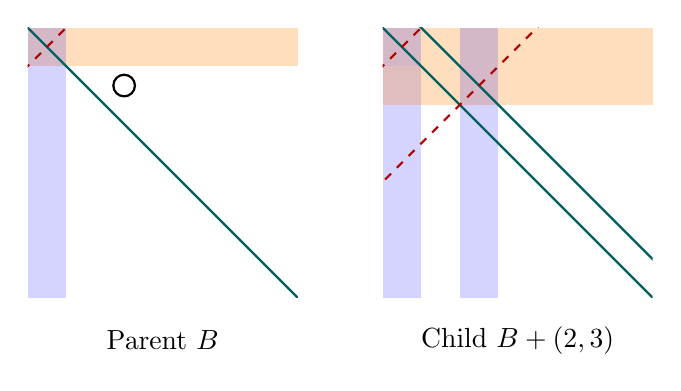
\begin{tikzpicture}[x=.49cm,y=.49cm]
 \foreach \etapa/\dx in {1/0,2/9.2}{
  \begin{scope}[shift={(\dx,0)}]
   \bcuadricula{7}
   \fill[orange,opacity=.26] (0,6) rectangle (7,7);
   \fill[blue,opacity=.17] (0,0) rectangle (1,7);
   \ifnum\etapa=2
    \fill[orange,opacity=.26] (0,5) rectangle (7,6);
    \fill[blue,opacity=.17] (2,0) rectangle (3,7);
   \fi
   \begin{scope}
    \clip (0,0) rectangle (7,7);
    \draw[teal!75!black,line width=.8pt] (.5,6.5) ++(-7,7) -- ++(14,-14);
    \draw[red!70!black,dashed,line width=.8pt] (.5,6.5) ++(-7,-7) -- ++(14,14);
    \ifnum\etapa=2
     \draw[teal!75!black,line width=.8pt] (2.5,5.5) ++(-7,7) -- ++(14,-14);
     \draw[red!70!black,dashed,line width=.8pt] (2.5,5.5) ++(-7,-7) -- ++(14,14);
    \fi
   \end{scope}
   \foreach \rr in {1,...,7}{
    \foreach \cc in {1,...,7}{
     \pgfmathtruncatemacro{\libre}{(\rr!=1)&&(\cc!=1)&&(abs(\rr-1)!=abs(\cc-1))}
     \ifnum\etapa=2
      \pgfmathtruncatemacro{\libre}{\libre&&(\rr!=2)&&(\cc!=3)&&(abs(\rr-2)!=abs(\cc-3))}
     \fi
     \ifnum\libre=1 \bmarca{7}{\rr}{\cc}\fi
    }
   }
   \breina{7}{1}{1}
   \ifnum\etapa=1
    \draw[black,line width=.8pt] (2.5,5.5) circle[radius=.28];
    \node at (3.5,-1.1) {Parent $B$};
   \else
    \breina{7}{2}{3}
    \node at (3.5,-1.1) {Child $B+(2,3)$};
   \fi
  \end{scope}
 }
\end{tikzpicture}
\caption{One transition from a parent to a child on a board of order seven. The parent has a queen
in row 1; the child is obtained by revealing row 2.
Rows are numbered from one, top to bottom, and columns from one, left to right. Crowns represent
queens already placed. The horizontal and vertical bands mark their occupied rows and columns.
Solid and dashed lines show the two families of diagonals under attack. Each dot marks an available
square. In the next row, row $2$, columns $3,4,5,6,7$ have $1,1,1,1,0$ completions, respectively,
so $Q(B)=4$. The circle marks the choice $(2,3)$ that gives the child on the right.}\label{fig:historia}
\end{figure}
